% !TeX root = ../presentation.tex

\section*{Introducción}
%----------------------------------------------------------------------------------
\begin{frame}{{Antecedentes}}

    \begin{alertblock}{Metasupeficies plasmónicas para biosensado}
        \begin{itemize}%[<+->]
         \itemsep9pt
         \item Arreglos bidimensionales de \textbf{nanoestructuras metálicas} (meta-átomos) soportadas por un sustrato.$^1$
        \end{itemize}
    \end{alertblock}
    
    \begin{center}
  	\begin{tikzpicture}[node distance=1em and 1em,font=\small]
        \path (0,0) node [flowbox] (bio) {\fbtitle{Meta-átomos}\vphantom{yÖ}
	    \nodepart{two}
         \begin{minipage}{.25\textwidth} \begin{itemize}
			\item Geometría
			\item Material
			\item Distribución
               \begin{itemize}
                  \item Desordenada $^{4,5}$
                  \item Periódica $^{2,3}$
               \end{itemize}
            \item \textbf{Perfecto soporte sobre sustrato}
         \end{itemize}\end{minipage}
        };

        \node[flowbox, below = of bio] (exp) {\fbtitle{Respuesta óptica}\vphantom{yÖ}
        \nodepart{two}
         \begin{minipage}{.25\textwidth} \begin{itemize}
            \item Resultados experimentales$^{2,3,4,5}$
            \item Simulaciones numéricas$^{2,3,4}$
            \item Teorías de medio efectivo$^5$
         \end{itemize}\end{minipage}
        };

        \node at (7,-1){\includegraphics[scale = .6]{background.png}};

        \node at (2.85, 1) {\ding{173}}; %2
        \node at (5.8,1.2) {\ding{174}};   %3
        \node at (6,-1.5) {\ding{175}}; %4
        \node at (9.6,1) {\ding{176}}; %5
    \end{tikzpicture}
    \end{center}   
    
    \vspace*{-4em}
    \begin{columns}
        \column{.35\textwidth}
        \column{.65\textwidth}
        \noindent\rule{.25\textwidth}{0.4pt}	
         \begin{spacing}{0}\fontsize{4}{12} \selectfont
            $^1$ \fullcite{gonzalez-alcalde_large_2020}\\
            $^2$ \fullcite{feuz_improving_2010}\\
            $^3$ \fullcite{kabashin_plasmonic_2009}\\
            $^4$ \fullcite{qiu_dual_2020}\\
            $^5$ \fullcite{svedendahl_refractometric_2014}
         \end{spacing}	
   \end{columns}
\end{frame}

%----------------------------------------------------------------------------------
\begin{frame}{{Objetivo}}
\begin{columns}
   \column{.55\textwidth}
   \begin{alertblock}{Incrustamiento parcial de meta-átomos en el sustrato}
        \begin{itemize}%[<+->]
         \item Resultados del proceso de fabricación$^1$
         \item Característica deseable para metasupeficies enfocadas para biosensado (Acoplamiento con sistemas de microfluídica)
         \item ¿Cuál es su efecto en la respuesta óptica?
        \end{itemize}
    \end{alertblock}
   \column{.45\textwidth}

   \begin{center}
  	\begin{tikzpicture}[node distance=1em and 1em,font=\small]
        \path (0,0) node [flowbox] (bio) {\fbtitle{Sistema de estudio}\vphantom{yÖ}
	    \nodepart{two}
         \begin{minipage}{.95\textwidth}
         Nanopartíula esférica apta para biosensado en metasuperficies\\

         \begin{itemize}
			\item Meta-átomo: 12.5 nm AuNP
			\item Matriz: Aire
			\item Sustrato: Vidrio
         \end{itemize}\end{minipage}
        };
    \end{tikzpicture}
    \end{center}
\end{columns}

    \begin{center}
  	\begin{tikzpicture}[node distance=1em and 1em,font=\small]
        \node at (0,0) {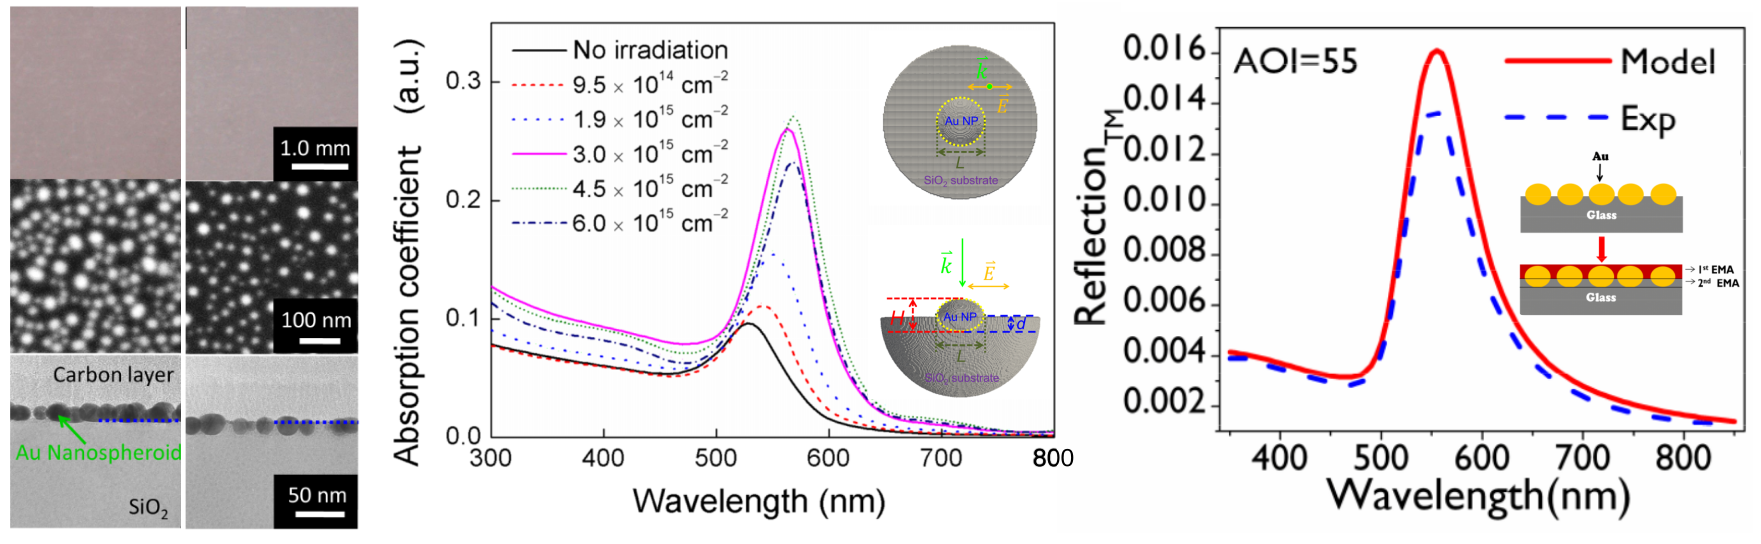
\includegraphics[scale = .7]{embedding.png}};

        \node at (-5.35,1.45) {\ding{172}}; %1
        \node at (1.25,1.35) {\ding{173}};   %2
    \end{tikzpicture}
    \end{center}

    \vspace*{0em}
        \noindent\rule{.25\textwidth}{0.4pt}
         \begin{spacing}{0}\fontsize{4}{12} \selectfont
            $^1$ \fullcite{meng_anisotropic_2015}\\
            $^2$ \fullcite{moirangthem_enhanced_2012}
         \end{spacing}
\end{frame}
